% ============================================================
% 分片：s03a  对应原文 PDF 第 33--36 页
% 负责章节：§3 Homotopy & further developments；3.1 Topological descent；
%           3.1.1 2d $A$- and $B$-models；3.1.2 3d $A$- and $B$-models
% 译者：translator-05   审校状态：初稿
% ============================================================

% ==== 原文 PDF 第 33 页 ====
% [说明: 第 33 页页首的正文段落（承接第 32 页末句 "There is an entire tower of higher
%  order products …"，止于 "the next section."）已按语义完整归入 s02h.tex 末尾；本分片
%  自第 33 页页首的 Figure 7 起。]

\begin{figure}[tbp]
  \centering
  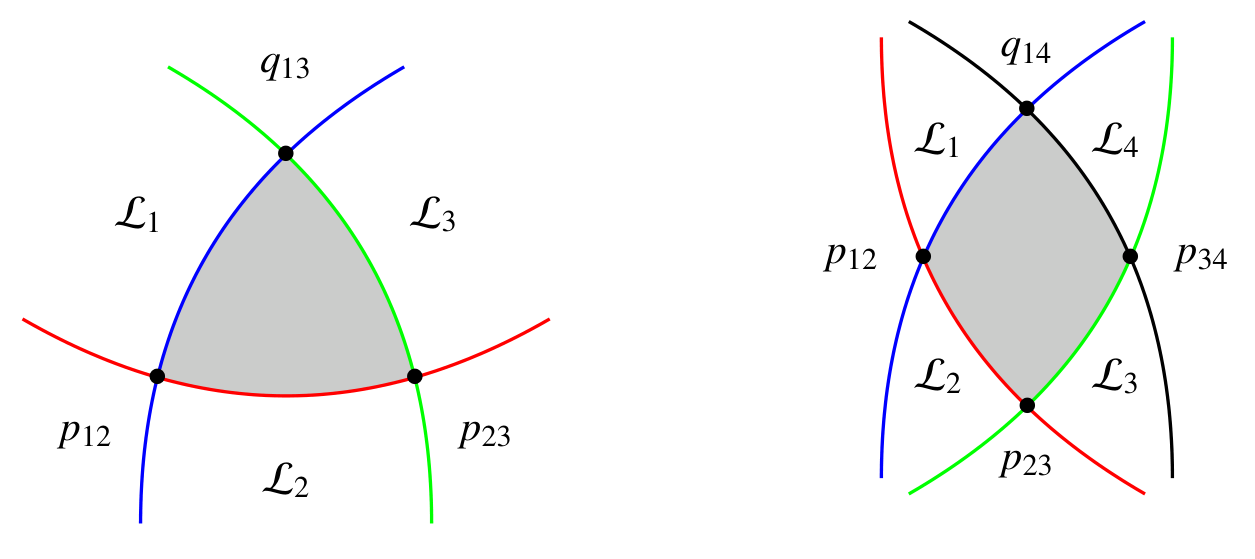
\includegraphics[width=0.95\linewidth]{figures/fig07.png}
  \caption{贡献于 Floer 乘积的全纯圆盘的图示。左：一个全纯圆盘，它贡献于二元 Floer 乘积 $|p_{12}\rangle\star|p_{23}\rangle$ 中 $|q_{13}\rangle$ 的系数。右：一个贡献于三元 Floer 乘积 $\mu_3(p_{12},p_{23},p_{34})$ 的全纯圆盘的图示。（原文第 33 页，Figure 7）}
\end{figure}

\section{同伦与若干后续发展}

\begin{keytakeaway}
\textbf{核心物理图像：}扭变使一部分超荷变成 1 形式的算符，它们把局域算子「下降」为形式值的算子；再把这些形式沿时空子流形积分，便得到支撑在子流形上的延展算子（线算子、面算子等）。这类 $Q$ 闭延展算子是匹配两个对偶（扭变）理论所需的算符。
\textbf{数学工具：}拓扑下降（descent）与下降方程 $QO^{(k)}=dO^{(k-1)}+(QO)^{(k)}$；用 $d$ 形式后代在时空上积分来构造作用量的形变；以及 $A_\infty$、$L_\infty$ 等同伦代数对「模去同伦的算子乘积」的刻画。
\textbf{主要结论：}由 Stokes 定理，$Q$ 闭局域算子的积分后代只依赖积分闭链的同调类（至多差 $Q$ 恰当项），故扭变理论只依赖有限个形变参数；延展算子与次级乘积给出这些形变与对偶关系的代数编码。
\end{keytakeaway}

本节讨论扭变理论的额外特征与丰富结构。这些考虑将引出同伦代数（homotopy algebra）的出现，粗略地说，它们刻画的是算子乘积在模去同伦之后的结构。为触及我们最关心的同伦结构，我们将越过上同调层面的局域算子代数，转而用链层面的考虑，通过称为下降（descent）的程序提取更精细的信息。这类链层面考虑的一个后果，是引入了一类自然的 $Q$ 闭延展算子（extended operator），它们是匹配两个对偶（扭变）理论之间物理的关键成分。这些延展算子最早出现在 Witten 对四维流形 Donaldson 不变量的研究中，其中他从四维流形中的非平凡 2-闭链计算出 2 形式后代 [17]。下降以及我们也将回顾的次级乘积（secondary product）概念，同样源于对弦世界面的基础性研究，例如 [49–51]。我们将解释下降程序，讨论这些延展算子存在性背后的代数结构，以及它们对局域算子本身的影响。这些结构在拓扑弦与弦场论的数学中起了重要作用，也在一些有趣的对偶中出现。

同伦代数的某些出现方式已为人熟知，特别是在镜像对称中，而后者来自世界面上的拓扑扭变。例如，关于镜像对称如何交换 $A$ 膜与 $B$ 膜的数学陈述，常以同伦代数与范畴的语言表述，参见 Kontsevich 的同调镜像对称（homological mirror symmetry）猜想 [41]。即便在扭变理论之外，同伦 Lie 代数（即 $L_\infty$ 代数）也作为基本要素出现在弦场论 [51–53] 与场论 [54] 中。其他同伦代数，特别是在全纯扭变理论中的那些，目前是数学与物理中活跃的研究方向；关于全纯场论的一般性讨论参见如 [55, 第 5 章]，关于三维混合全纯–拓扑理论的详细讨论参见 [56, 第 2 节]。
% [跨页接续: 原文第33页/第34页——本段末句自第 33 页末行 "…in mathematics and physics;" 跨至
%  第 34 页首行 "see e.g. [55, Chapter 5] …"，已按语义完整置于本段末]

% ==== 原文 PDF 第 34 页 ====
\subsection{拓扑下降}

继续考虑拓扑扭变理论的情形（包括扭变同态 $\iota$ 的选取）。与之前一样，$A$ 模型与 $B$ 模型将作为我们的主要例子。本小节大体上继续沿用 [9] 的记号与表述。在 2.3 节，我们简要导出了关于如今已为标量的超荷 $Q_B$ 与 $Q_A$ 的 $Q$ 上同调中的局域（即零形式）算子代数，或说手征环与扭手征环。其余超荷的自旋也被扭变所改变：它们成为 1 形式。这一特点使我们能在拓扑扭变理论中考虑更广一类的形式值可观测量。粗略地说，它们由把局域算子下降为微分形式值的算子、再把这些形式在适当的时空子流形上积分而得到。这一程序称为拓扑下降（topological descent）。\footnote{你或许在学习 $2n$ 维场论的 $2n+2$ 形式值反常多项式时见过下降方程的某个版本。反常多项式上的一个下降方程版本可用来在时空上生成 $2n$ 形式局域抵消项。抵消项的歧义在下降的观点下表现为上同调的恰当性。细节参见如 [57]。}

下面显式地看这一点。任意维数下，一个基本的扭变\footnote{由于在这一分析中我们并不要求更强的「能动张量为 $Q$ 恰当」这一条件，这些理论可以称为弱拓扑扭变的（weakly topologically-twisted）。}超 Poincaré 代数具有如下形式：有幂零的扭变超荷 $[Q,Q]=0$；有沿 $x^\mu$ 生成平移的动量 $P_\mu \sim -i\partial_\mu$，它们彼此对易 $[P_\mu,P_\nu]=0$ 且为 $Q$ 闭 $[Q,P_\mu]=0$；还有超荷 $Q_\mu$，它们必然与动量对易 $[Q_\mu,P_\nu]=0$、彼此对易 $[Q_\mu,Q_\nu]=0$，并保证动量是 $Q$ 恰当的 $[Q,Q_\mu]=iP_\mu$。给定一般算子 $O(x)$，可以定义其 1 形式拓扑后代（topological descendant）：
\begin{equation}\tag{3.1}
O^{(1)}(x) := -dx^\mu O_\mu(x),\qquad O_\mu(x) = [Q_\mu,O(x)]\,.
\end{equation}
% [Tutor Note: 这里 $O_\mu=[Q_\mu,O]$ 是下降的第一步：$Q_\mu$ 是自旋被扭变改造过的超荷，它带一个形式指标 $\mu$，因此作用在零形式算子上给出 1 形式。上标 $(1)$ 记录形式次数，而非某个新的物理荷。]

利用扭变 Poincaré 代数，1 形式值的算子 $O^{(1)}$ 满足下式
% [版式说明: 原文 (3.2) 排为两行；因 A4 版心较原文窄，此处拆为三行（内容、符号与编号均不变），以避免 overfull hbox。]
\begin{equation}\tag{3.2}
\begin{aligned}
QO^{(1)} &= -[Q,dx^\mu[Q_\mu,O]]\\
&= dx^\mu\big(i[P_\mu,O] - [Q_\mu,[Q,O(x)]]\big)\\
&= dO + (QO)^{(1)}\,,
\end{aligned}
\end{equation}
其中 $d = dx^\mu\partial_\mu$ 是时空外微分。
% [Tutor Note: 中间一步的代数来源：用（分次）Jacobi 恒等式展开 $[Q,[Q_\mu,O]]$，再用原代的 $[Q,Q_\mu]=iP_\mu$ 把它换成 $iP_\mu$ 与 $[Q_\mu,[Q,O]]$ 的组合，即得 $dx^\mu\big(i[P_\mu,O]-[Q_\mu,[Q,O(x)]]\big)$；其中 $dx^\mu i[P_\mu,O]=dO$（因 $P_\mu\sim-i\partial_\mu$），第二项按定义就是 $(QO)^{(1)}$。具体符号取决于分次括号的约定，核对时应与原文的 $[Q,Q_\mu]=iP_\mu$ 保持一致。式 (3.2) 正是「下降」这一名称的来源：$Q$ 与 $d$ 在同调层面互换角色。]
可见若 $O$ 为 $Q$ 闭（$QO=0$），其第一个后代 $O^{(1)}$ 并不 $Q$ 闭，而是显式地包含了 $O$ 对位置的依赖信息。特别地，若选取从 $x$ 到 $y$ 的路径 $\gamma_{x\to y}$，可以如下定义延展算子
\begin{equation}\tag{3.3}
O(\gamma_{x\to y}) = \int_{\gamma_{x\to y}} O^{(1)}\,.
\end{equation}
下降方程连同 Stokes 定理表明：$O(\gamma_{x\to y})$ 的 $Q$ 变分实现了 $O$ 在 $Q$ 上同调中的位置无关性，即 $QO(\gamma_{x\to y}) = O(y)-O(x)$。
% [Tutor Note: 这一步是 Stokes 定理的直接应用：$\int_\gamma QO^{(1)} = \int_\gamma dO = O(y)-O(x)$。它在物理上意味着：$Q$ 闭算子的关联函数与插入点的位置无关（至多差 $Q$ 恰当项），这正是一类拓扑不变量的代数基础。]

% ==== 原文 PDF 第 35 页 ====
可以对更高形式的后代继续这一过程：
\begin{equation}\tag{3.4}
\begin{aligned}
O^{(2)}(x) &= \frac{1}{2}dx^\mu\wedge dx^\nu[Q_\mu,[Q_\nu,O(x)]]\\
&\quad\vdots\\
O^{(k)}(x) &= \frac{(-1)^k}{k!}dx^{\mu_1}\wedge\ldots\wedge dx^{\mu_k}
[Q_{\mu_1},[\ldots,[Q_{\mu_k},O]]]\,.
\end{aligned}
\end{equation}
同样，即使 $O$ 为 $Q$ 闭，这些后代也不 $Q$ 闭；它们满足下降方程：
\begin{equation}\tag{3.5}
QO^{(k)} = dO^{(k-1)} + (QO)^{(k)}\,.
\end{equation}
可以把 $k$ 形式后代 $O^{(k)}(x)$ 在时空的 $k$ 维子流形 $\gamma$ 上积分，得到支撑在 $\gamma$ 上的延展算子 $O(\gamma)$；下降方程保证：当 $O$ 为 $Q$ 闭时，所得算子只依赖于积分闭链的同调类（至多差 $Q$ 恰当项）：Stokes 定理给出 $Q(O(\gamma)) = O(\partial\gamma)$。特别地，若把这些后代在非平凡 $k$-闭链（即满足 $\partial\gamma=0$ 的 $\gamma$）上积分，所得的延展算子 $O(\gamma)$ 必然 $Q$ 闭。
% [Tutor Note: (3.4) 的归一化值得核对：$1/k!$ 来自 $k$ 个指标 $\mu_1,\ldots,\mu_k$ 的全排列（wedge 已给出反对称化，故每个排列只应计一次）；$(-1)^k$ 则来自逐次移动奇鬼数的 $Q_\mu$ 因子所产生的符号，须与本节所用的分次括号约定一致。若漏掉 $1/k!$，高阶后代就会比 (3.4) 大 $k!$ 倍。]

\subsubsection{二维 $A$ 型与 $B$ 模型}

在诸如 $B$ 模型这样的二维理论中，有 1 形式与 2 形式的后代，可以在各种拓扑的世界面上研究，它们由下式给出
\begin{equation}\tag{3.6}
\begin{aligned}
O^{(1)} &= -\frac{1}{2i}dz[Q_-,O] + \frac{1}{2i}d\bar z[Q_+,O]\\
O^{(2)} &= \frac{1}{4}dz\wedge d\bar z[Q_-,[Q_+,O]]
\end{aligned}
\end{equation}
而在 $A$ 模型中为
\begin{equation}\tag{3.7}
\begin{aligned}
O^{(1)} &= -\frac{1}{2i}dz[\bar Q_-,O] + \frac{1}{2i}d\bar z[Q_+,O]\\
O^{(2)} &= \frac{1}{4}dz\wedge d\bar z[\bar Q_-,[Q_+,O]]
\end{aligned}
\end{equation}
% [Tutor Note: 比较 (3.6) 与 (3.7)：$B$ 模型用 $Q_-$，$A$ 模型用 $\bar Q_-$，而 $d\bar z$ 一项两者的系数都取 $Q_+$。若把 $A$ 模型的 $\bar Q_-$ 误写成 $Q_-$，得到的延展算子将不再与相应的扭变超荷对易，形变论证随之失效——这是核对 $A/B$ 模型下降公式时最易出错之处。]

在 $d$ 维 TQFT 中，$d$ 形式后代实际上支配着原 TQFT 的有趣形变。理由很简单：可以把 $d$ 形式后代在（欧氏）时空上积分，并把结果（乘以任意耦合常数）加到原作用量上。当 $O$ 为 $Q$ 闭时，所得的积分后代（在闭合时空上，或给定适当的边界条件时）也为 $Q$ 闭，因此它（至少在经典层面）代表原作用量的一个自洽形变。
% [原文疑误: 原文 "one can can integrate the $d$-form descendants" 中 "can" 重复一次；译文只译一处，其余未改。]

例如，在依赖于手征参数的 $B$ 模型中，对应于超势形变的项可以通过考察手征算子 $\delta W(\phi)$ 的 2 形式后代得到。具体地，超势的形变可以写成 $\int d^2z\,d^2\theta\,\delta W(\Phi)$，它在超空间坐标上积分后给出一个正比于 $\int d^2z\,[Q_-,[Q_+,\delta W(\phi)]] \sim \int (\delta W(\phi))^{(2)}$ 的项，而这正是对应于超势形变的手征算子的 2 形式后代。在 $B$ 模型中也可作类似操作，证明 $D$ 项形变与扭 $F$ 项形变是 $Q_B$ 恰当的，因而不对应于后代。如所预期，$A$ 模型中有类似结论：扭手征算子的 2 形式后代支配该模型的形变，而 $D$ 项与 $F$ 项形变是 $Q_A$ 恰当的。
% [Tutor Note: 这里把 (3.6) 的 $O^{(2)}=\frac14 dz\wedge d\bar z[Q_-,[Q_+,\cdot]]$ 直接用于 $\delta W(\phi)$，即得 $\int d^2z[Q_-,[Q_+,\delta W(\phi)]]=\int(\delta W(\phi))^{(2)}$；这也解释了为何超势形变（$F$ 项）在 $B$ 模型中由 2 形式后代给出，而 $D$ 项形变是 $Q_B$ 恰当的——后者的形变参数不是手征参数。]

% ==== 原文 PDF 第 36 页 ====
如 [9] 及其文献所强调的，这些扭变理论的一个美妙之处在于：扭变使我们能够集中考察可能的形变中一个可处理的有限子集。完整物理（即未扭变）理论中的一般关联函数会依赖于无穷多个参数。扭变的上同调性质的一个后果是：扭变后的关联函数只依赖于我们所考虑的、对世界面理论作微扰的有限个参数（分别为 $F$ 项或扭 $F$ 项）。乘在这些形变项上的耦合常数可以解释为物理理论的模空间上的局部坐标。

在 $\mathcal{N}=(2,2)$ 超共形场论的情形，由严格边缘形变张成的共形流形在局部可分解为两个（凯勒）流形的乘积，它们分别对应手征形变与扭手征形变。这两个因子正是分别由 $B$ 型与 $A$ 型扭变所触及的形变；当这些超共形场论是以 Calabi–Yau 为靶空间的 $\sigma$ 模型时，这两个局部因子分别与 Calabi–Yau 几何的复结构模空间和凯勒模空间重合。从手征环的性质出发研究这些模空间几何的一些文献包括 [58–61]。\footnote{注意并非所有扭变都局域化在「可解释为模空间上向量丛的截面」的算子上。例如，二维 $\mathcal{N}=(4,4)$ 超共形场论中的 $1/4$-BPS 算子——它们可以很自然地在全纯（或半扭变）框架下研究——给出模空间上的层（sheaf）：其秩（即这类算子的数目）可能在理论获得更强对称性的模空间子轨迹上不连续地跳变。\par 为说明这一现象，下面给出一个与本文主题密切相关的更简单的例子：考虑只含单个手征多重态 $\Phi$ 的 Landau–Ginzburg 模型（凯勒靶空间是平坦复平面 $\mathbb{C}$），其超势为 $n$ 阶，即 $W = \Phi^n + \ldots$。对一般的超势，该理论有 $n-1$ 个真空，由 $W$ 的各不相同临界点标记，从而给出 $n-1$ 个基本 $A$ 膜。然而在共形点 $W = \Phi^n$ 处，它有 $\binom{n}{2}$ 个基本 $A$ 膜，对应于 $\mathbb{Z}/n\mathbb{Z}$ 增强对称性。关于这一例子的更多细节参见 [62, 第 5.2 节]。}

\subsubsection{三维 $A$ 型与 $B$ 模型}

三维 $\mathcal{N}=4$ 超 Poincaré 代数在许多方面与这些讲义中已详述的二维 $\mathcal{N}=(2,2)$ 代数相似。该代数有 8 个超荷，我们记之为 $Q_\alpha^{a\dot a}$，其中 $\alpha\in\{\pm\}$ 是 $Spin(3)\cong SU(2)$ 的自旋指标，$a\in\{\pm\}$、$\dot a\in\{\pm\}$ 是 $SO(4)\cong (SU(2)_A\times SU(2)_B)/\mathbb{Z}_2$ 的 $R$ 对称性指标。在没有中心荷时，反对易子可表为
\begin{equation}\tag{3.8}
[Q_\alpha^{a\dot a},Q_\beta^{b\dot b}]
= \epsilon^{ab}\epsilon^{\dot a\dot b}(\sigma^\mu)_{\alpha\beta}P_\mu
\end{equation}
其中 $(\sigma^\mu)^\alpha{}_\beta$ 为 Pauli 矩阵。（三维自旋指标用 Levi-Civita 张量 $\epsilon^{\alpha\beta}$ 升降。）
% [Tutor Note: 指标位置须逐一对齐：$\alpha,\beta$ 是 $Spin(3)$ 自旋指标，$a,b$ 与 $\dot a,\dot b$ 分别是两个 $SU(2)\subset SO(4)$ 的 $R$ 对称指标。$\epsilon^{ab}\epsilon^{\dot a\dot b}$ 同时缩并这两组 $R$ 指标，故右端对 $a,b,\dot a,\dot b$ 是反对称的；若误把 $\dot a$ 与 $a$ 当作同一指标处理，就会破坏这一结构。另注意正文用 $(\sigma^\mu)^\alpha{}_\beta$，而式 (3.8) 用 $(\sigma^\mu)_{\alpha\beta}$，两者相差一次用 $\epsilon^{\alpha\beta}$ 的升降。]

在两个超对称代数中，$R$ 对称性群都（局部）同构于欧氏自旋群的两份拷贝，即 $\mathfrak{g}_R \cong \operatorname{spin}(d)\oplus\operatorname{spin}(d)$，并带有一个交换这两个 $R$ 对称性的镜像自同构（mirror automorphism）。因此，这些超对称代数中的每一个都容许两个不同的完全拓扑扭变，它们在该代数的这个自同构下互换。与二维情形类比，三维 $\mathcal{N}=4$ 理论的两个拓扑扭变被称为
\footnote{历史上，我们所称的 $B$ 型扭变即 Rozansky–Witten 扭变，得名于被称为 Rozansky–Witten 理论的三维 TQFT [63]；但这一扭变也由 Blau 与 Thompson 在纯规范理论中研究过 [64]。我们所称的 $A$ 型扭变在历史上称为镜像 Rozansky–Witten 扭变，是 [17] 中四维 Donaldson–Witten 扭变的维数约化。本文采用的名称反映了这样一个事实：三维的 $A$ 型与 $B$ 型扭变在三维体的二维 $\mathcal{N}=(2,2)$ 边界上分别成为二维的 $A$ 型与 $B$ 型扭变。类似地，三维的 $A$ 型与 $B$ 型扭变可以位于四维 $\mathcal{N}=4$ 的 $A$ 型与 $B$ 型扭变的边界上，而后者本身是 [65] 中 Kapustin–Witten 扭变或 Langlands 扭变的 $\psi\to 0,\infty$ 极限。}
$A$ 型与 $B$ 型扭变，其
% [跨页接续: 原文第36页/第37页——原句至第 36 页末 "…are called the $A$ and $B$ twists with" 处被页边界截断，
%  其后半段属 s03b.tex 起始内容（该分片以「扭变超荷例如为 $Q_A=\ldots$」开篇）；此处的「，其」对应原文的 "with"，
%  与 s03b 开篇连读为「……，其扭变超荷例如为……」。切勿在本分片补句。]
